% Introduction to the problem
% - which MIs need to be evaluated
% - which are impossible to evaluate analitically
% - How we proceeded

\section{Two-loop MIs for the neutral-current Drell-Yan}
\label{sec:results}

As a first practical application of the algorithm discussed in section \ref{sec:series}, we provide the results for the evaluation of the MIs relevant for the mixed QCD-EW corrections to the neutral-current Drell-Yan process, recently presented in Ref \cite{Armadillo:2022bgm}. 
%
We focus on the integrals numbered 32-36 in Ref.~\cite{Bonciani:2016ypc},
because their complexity offers an interesting case to study the performances of our new package. The solution proposed in Ref.~\cite{Bonciani:2016ypc} in terms of Chen-Goncharov repeated integrals has severe limitations in the numerical evaluation in the physical region, and a semi-analytical approach represents an interesting alternative.
%For all of them a closed analytic expression exists \cite{Bonciani:2016ypc,Heller:2019gkq}. However, for the five most challenging MIs this analytic expression is not publicly available.

We first introduce the problem, then we show a comparison between the solution obtained with real and complex internal masses, and, finally, we discuss the numerical and time performances of our code. 

\subsection{Master integrals for the mixed EW-QCD corrections to the neutral-current Drell-Yan}

The NNLO mixed QCD-EW corrections to the neutral current Drell-Yan have been calculated recently in Ref. \cite{Armadillo:2022bgm}.
In the complete amplitude 204 MIs appear and they can be evaluated using the method of differential equations. 

These integrals can be classified into three different groups \cite{Bonciani:2016ypc}, according to the number of their internal massive lines: zero, one or two. 
The four-point functions corresponding to the first two sets are known in closed analytic form in terms of generalized polylogarithms (GPLs).
%are well-known in the literature. 
The last group
%, on the contrary, 
is 
%very 
the most challenging due to the presence of different kinematic scales. 
In particular 36 MIs belong to this set.
For 31 of them, a solution in terms of GPLs is known. 
The remaining 5 have been formally solved in \cite{Bonciani:2016ypc} using a formal expression in terms of Chen-Goncharov integrals \cite{Chen:1977oja}.
%}
% These integrals belong to the family indicated as $B_{16}$ and $B_{16p}$ in Ref. [x], that is 
% \begin{align}
%     {\rm B}_{16} &: \{ \cD_1, \cD_2-\mu_V^2, \cD_{12}, \cD_{1;1}, \cD_{2;1}, \cD_{1;12}, \cD_{2;12}-\mu_V^2, \cD_{1;3}, \cD_{2;3} \},
%               \nonumber\\
%     {\rm B}_{16p} &: \{ \cD_1, \cD_2-\mu_V^2, \cD_{12}, \cD_{1;2}, \cD_{2;2}, \cD_{1;12}, \cD_{2;12}-\mu_V^2, \cD_{1;3}, \cD_{2;3} \},
% \end{align}
These MIs belong to the following integral family (see the classification in \cite{Armadillo:2022bgm}):
\be
\{ \cD_1, \cD_2-m_V^2, \cD_{12}, \cD_{1;1}, \cD_{2;1}, \cD_{1;12}, \cD_{2;12}-m_V^2, \cD_{1;3}, \cD_{2;3} \}
\ee
where $V$ can be either $W$ or $Z$ and $m^2_V$ is the mass-squared of the $V$ boson. We defined $\cD$s to be:
\be
    \cD_{i} = k_{i}^2,\;
    \cD_{ij} = (k_i-k_j)^2,\;
    \cD_{i;j} = (k_i-p_j)^2,\;
    \cD_{i;jl} = (k_i-p_j-p_l)^2,
\ee
where $p_i$ are the external momenta and $k_j$ the loop ones.
In particular the 5 MIs are:
\begin{align}
    &\text{Master 32}\;:\:\{0, 1, 1, 1, 0, 1, 1, 0, 1\} \quad &&\text{Master 33}\;:\:\{1, 1, 1, 1, 0, 1, 1, 0, 1\} \nonumber\\
    &\text{Master 34}\;:\:\{1, 1, 1, 1, -1, 1, 1, 0, 1\} \quad &&\text{Master 35}\;:\:\{1, 1, 1, 1, 0, 1, 1, -1, 1\}\nonumber\\
    &\text{Master 36}\;:\:\{1, 1, 1, 1, -1, 1, 1, -1, 1\}\;,
\label{eq:difficultMIs}
\end{align}
where we keep the numbering from Ref. \cite{Armadillo:2022bgm}.\
It is possible to numerically evaluate the Chen iterated integrals in the Euclidean region, where the boundary conditions are imposed.
Their analytic continuation in the physical region, however, is non trivial and no standard technique to perform it is available. For this reason their computation in Ref.\cite{Armadillo:2022bgm} has been performed by using a semi-analytical approach, that is by solving the relevant system of differential equations using a series expansion method as described in Section \ref{sec:series}. 
By approaching the numerical evaluation of these MIs in such a semi-analytical way, we have to solve the complete system (36x36) of differential equations which includes the integrals from eq. \ref{eq:difficultMIs}.

These MIs depend on two dimensionless kinematic invariants
$x$ and $y$:
\be
    s=(p_1+p_2)^2 \;,\qquad
    t=(p_1-p_3)^2 \;,\qquad
    x=-\frac{ s }{ M^2 }\;,\qquad
    y=-\frac{ t }{M^2 }\;,
    \label{eq:kinVariablesReal}
\ee
where $p_{1,2}$ are incoming momenta, $p_3$ is an outgoing momentum, $s,t$ are the Mandlestam invariant, and
$M$ is the mass of the vector boson.
Let us consider first the case of real-valued masses $M=m_V$, with $V=W,Z$.

% The steps for evaluating the solution can be, hence, summarised as follows:
% \begin{itemize}
% 	\item choose the value of the physical $(\sqrt{s}, \; \cos\theta)$ for which we would like to evaluate the solution and using eq. \ref{eq:kinVariablesReal} and \ref{eq:relationTCostheta} compute the corresponding value for the dimensionless variable $(s,\;t)$,
% 	\item perform the analytic continuation of the solution from the point in which the boundary conditions are imposed to $(s,\;t)$ using the algorithm presented in Section \ref{sec:series}.
% \end{itemize}
% The last step can be performed using \texttt{SeaSyde} in a straight-forward way:
Once we have chosen the point $(x,y)$
%, or equivalently $(\sqrt{s},\cos\theta)$, 
in which we would like to evaluate the solution, the latter can be obtained in a straightforward way
%\footnote{For consistency with Ref.~\cite{Bonciani:2016ypc}, we define $x=-\tilde s$ and $y=-\tilde t$. }
using \textsc{SeaSyde}:
% $\overset{\verb!~}{\verb!s}$
%, codes={\catcode`$=3\catcode`^=7}]
\begin{Verbatim}[commandchars=\\\{\}] 
ConfigurationNCDY=\{                               
	EpsilonOrder->4,                               
	ExpansionOrder->50                                 
\};                                                      
UpdateConfiguration[ConfigurationNCDY];

SetSystemOfDifferentialEquation[SystemOfEquations, 
	        BoundaryConditions, MIs, \{x-I\textdelta,y+I\textdelta\}, pointBC]; 

TransportBoundaryConditions[ \{ tValue , sValue \} ]

SolutionValue[]
\end{Verbatim}

We use in this case a form of the MIs in which they are re-scaled by a power of $\varepsilon$, so that they do not contain explicit divergences in $\varepsilon$. 
Due to this re-scaling, in order to obtain the finite part for MI32-36 listed in Eq. \ref{eq:difficultMIs} we need to keep 5 terms in the $\varepsilon$ expansion.
% In order to bring the system in canonical form, some master integrals have been scaled by a factor $\varepsilon^k$, with $k=1,2,3,4$. The final system goes from $\mathcal{O}(\varepsilon^0)$ to $\mathcal{O}(\varepsilon^4)$. The choice to expand up to $\mathcal{O}(\varepsilon^4)$ is necessary in order to obtain the finite part for MI32-36 listed in eq. \ref{eq:difficultMIs}.
We have chosen to keep 50
terms in the expansion with respect to the kinematical variable, because it is a good compromise between execution time and precision; we will comment later 
how the number of terms affects the numerical precision. In \texttt{SetSystemOfDifferentialEquation} 
we are preparing the package for solving the system and, finally, using \texttt{Transport\-Boundary\-Conditions}
we are both solving the system and performing the analytic continuation, which let
us extend the solution from \texttt{pointBC}, where the boundary conditions are imposed, to \texttt{x=sValue} and 
\texttt{y=tValue}. At this point, by calling again the routine \texttt{Transport\-Boundary\-Conditions} we could transport the boundary conditions from \texttt{\{x=sValue, y=tValue\}} to 
\texttt{\{x=sValueNEW, y=tValueNEW\}} and so on. By repeating this procedure multiple times we can easily obtain a numerical grid for all the MIs. In \ref{app:packagedoc} we provide the full documentation of the package.

\subsection{Feynman integrals with complex-valued masses}

When dealing with intermediate unstable particles, such as $W$s and $Z$s, it is useful to perform the calculations in the CMS, in order to regularise the behaviour at the resonance while preserving the gauge invariance of the scattering amplitude.
To this end, we introduce the complex mass, defined as:
\be 
\label{eq:complex_mass}
\mu^2_V = m_V^2 - i \Gamma_V m_V,
\ee
where $\Gamma_V$, a real parameter, labels the decay rate of the boson.
The complex mass $\mu_V$ then replaces the real mass $m_V$ in all the steps of the computation.
From Eq.~(\ref{eq:kinVariablesReal}), in particular, we can observe that the
dimensionless kinematic variables $x$ and $y$ become complex-valued, once we set $M=\mu_V$.

The complex mass regularises the integrand function in the threshold region: indeed, all the propagators
\be
	\frac{1}{s-\mu_V^2+i\delta}
\ee
do not diverge for any real value of $s$, and, hence, in the kinematic region near the resonances, the MIs are smooth functions.

This fact let us really appreciate the discussion about the analytic continuation in the complex plane presented in Section \ref{sec:series}:
thanks to the algorithm for performing the analytic continuation of the solution included in {\sc SeaSyde}, we are able to evaluate the 5 MIs of interest at every point of the physical region and for arbitrary complex variables, thus implementing the CMS in a straightforward way.

\begin{figure}[ht!]
    \centering
    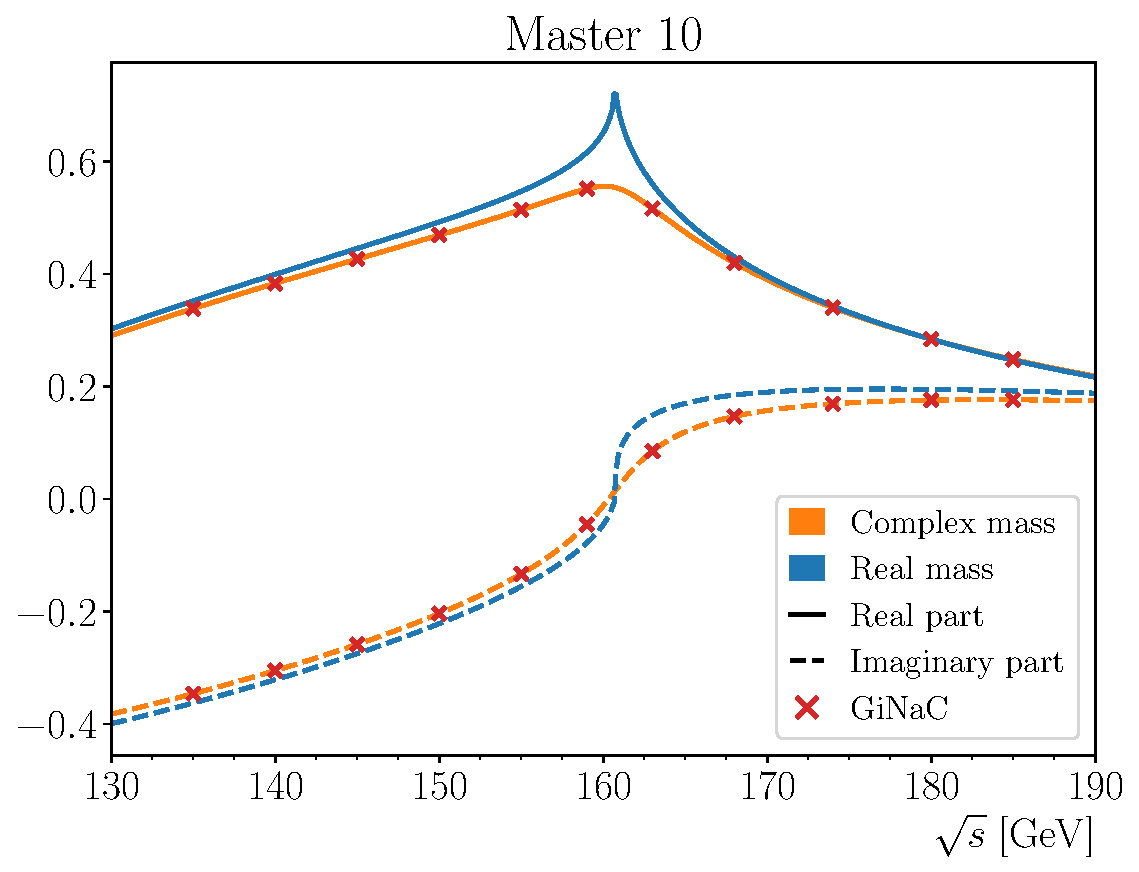
\includegraphics[width=0.45\textwidth]{paperSeaFire/Images/master10_legend.pdf}
    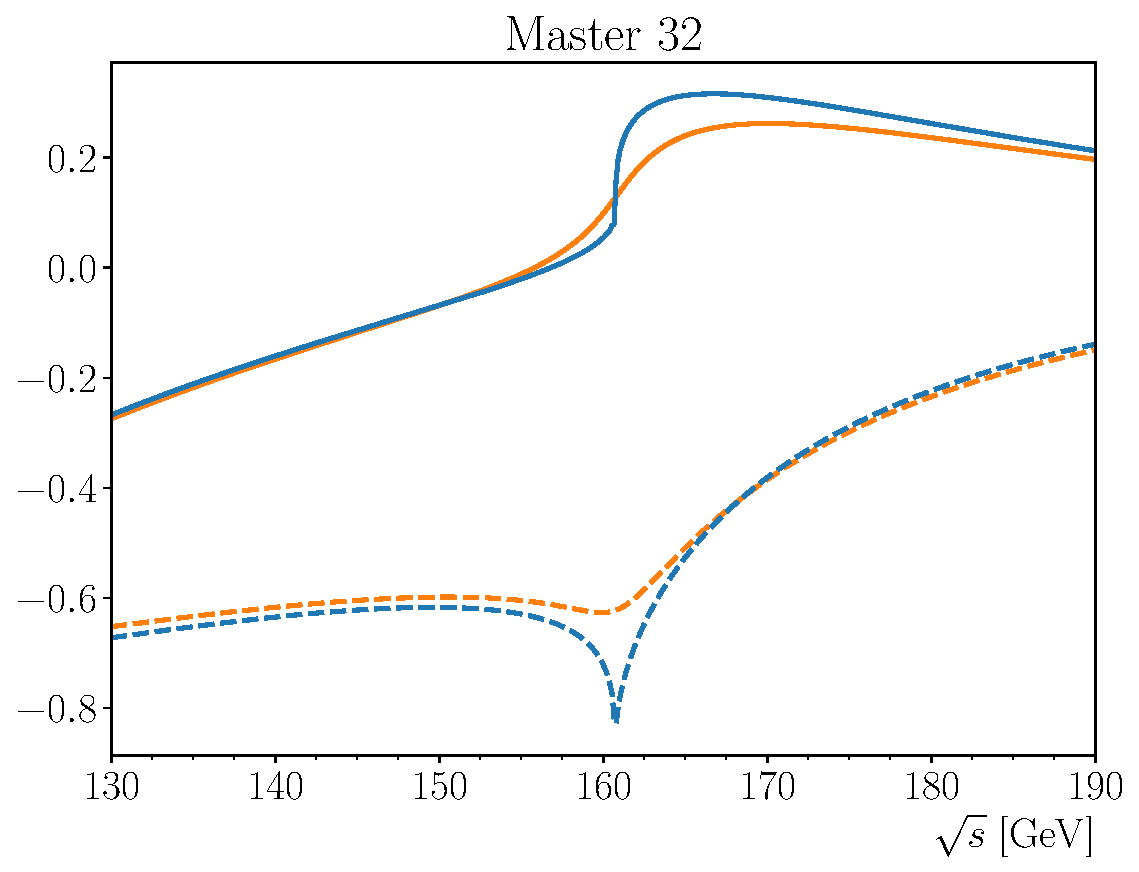
\includegraphics[width=0.45\textwidth]{paperSeaFire/Images/master32.pdf}
    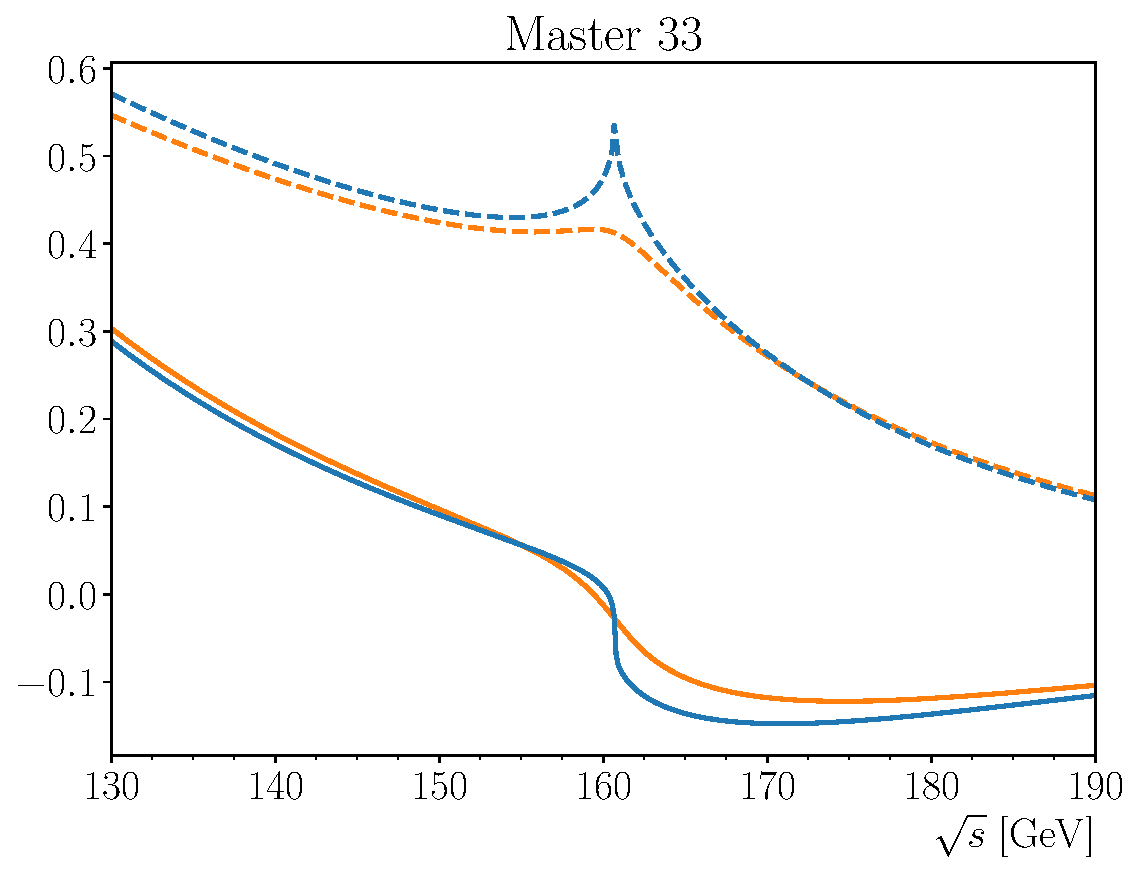
\includegraphics[width=0.45\textwidth]{paperSeaFire/Images/master33.pdf}
    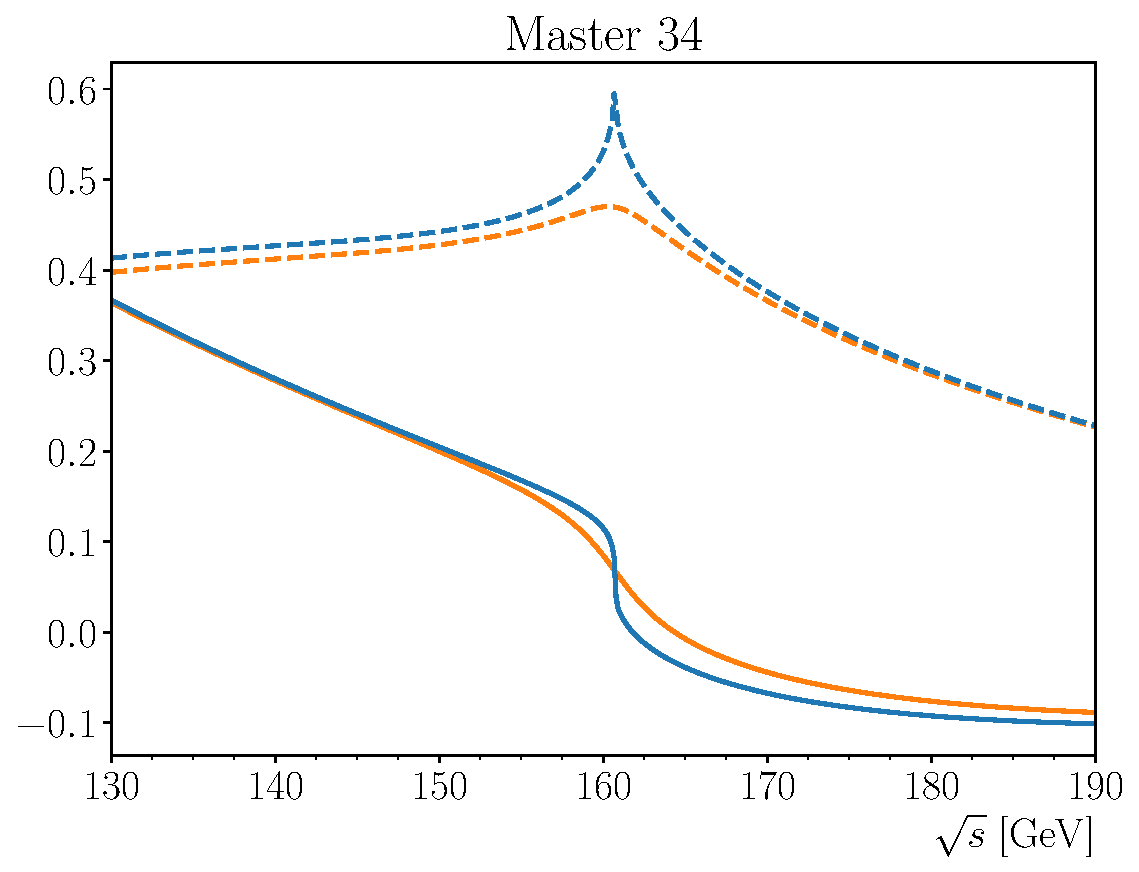
\includegraphics[width=0.45\textwidth]{paperSeaFire/Images/master34.pdf}
    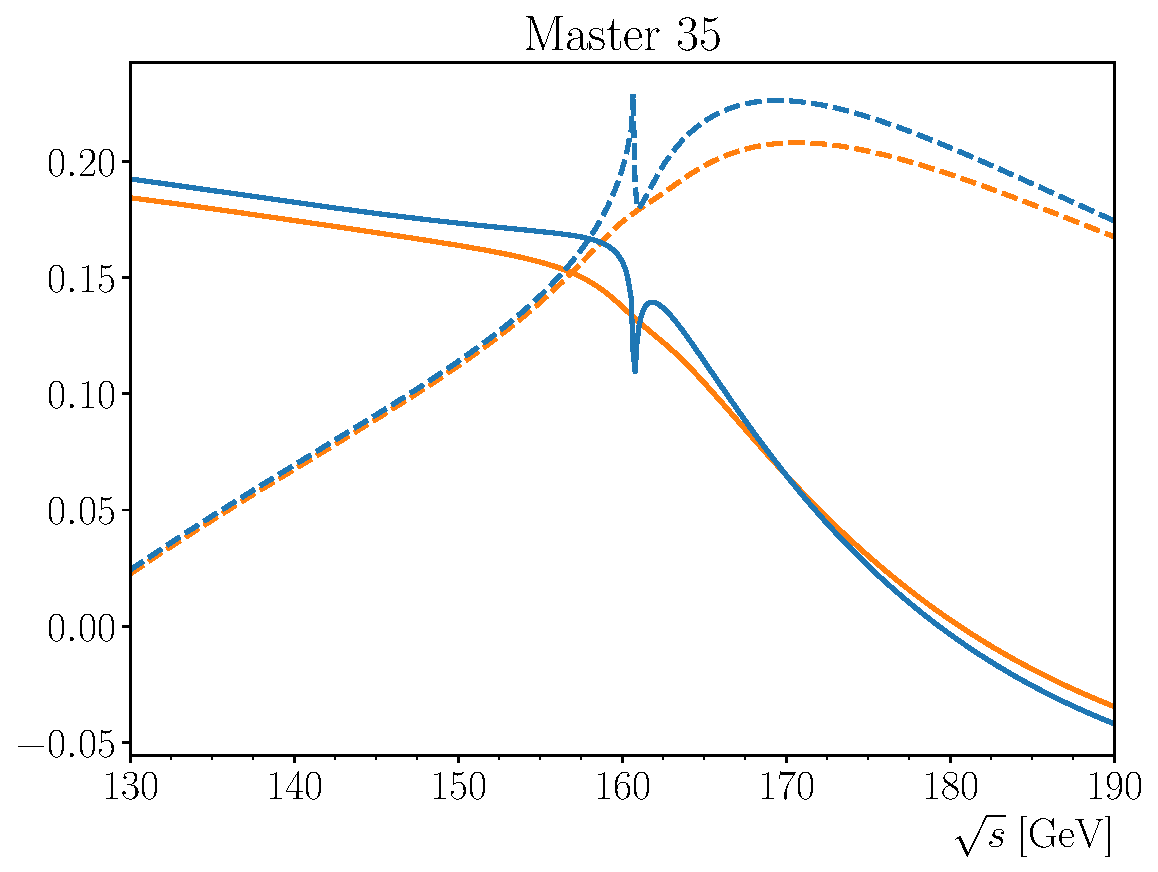
\includegraphics[width=0.45\textwidth]{paperSeaFire/Images/master35.pdf}
    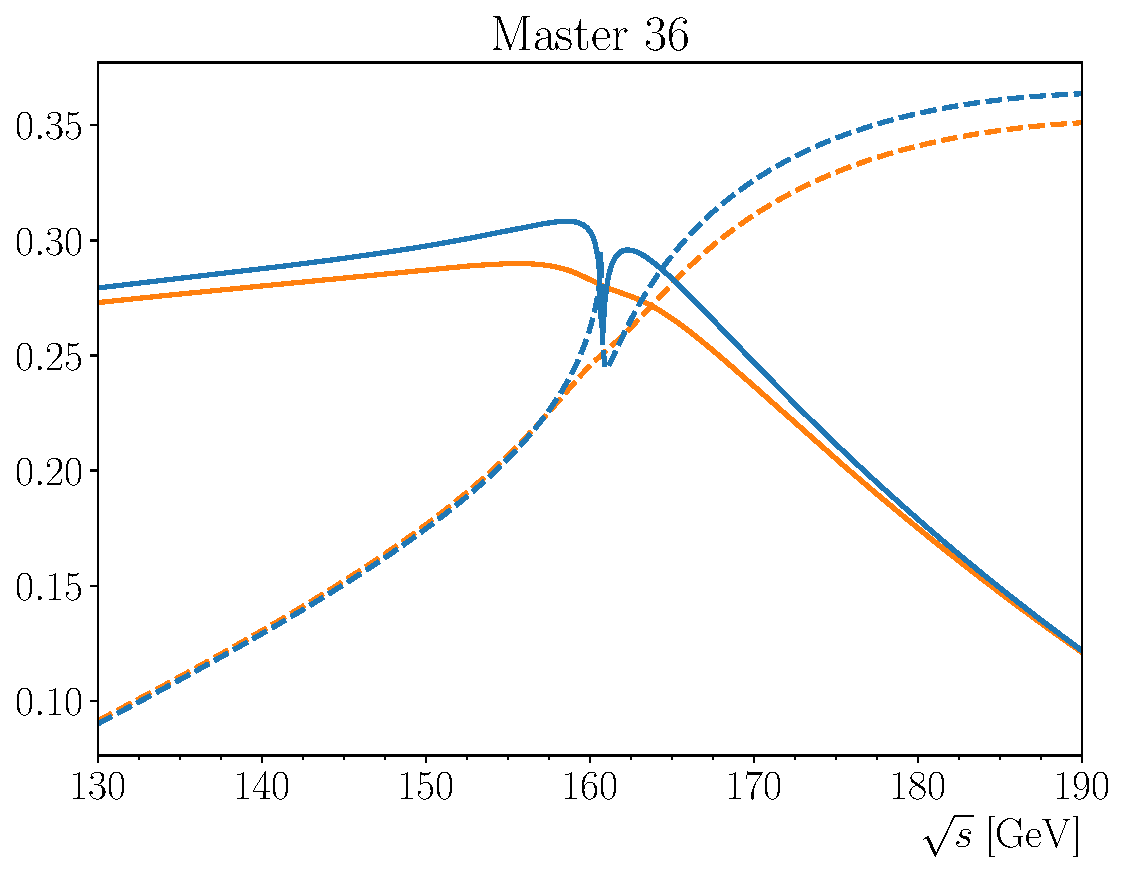
\includegraphics[width=0.45\textwidth]{paperSeaFire/Images/master36.pdf}
    \caption{Comparison between real- and complex-valued masses for MI10 and MIs from 32 to 36. The plots show the value of the $\varepsilon^0$ order  for $130 \; \text{GeV} \le \sqrt{s} \le 190\;\text{GeV}$, $\cos\theta=0$ and $M^2=m_W^2$ or $M^2=\mu_W^2$. 
    %The blue lines represent the masters for real-valued masses, while the orange the complex-valued ones. The solid and dashed lines represent the real and imaginary part of the solution, respectively. 
    In the MI10 plot, the red crosses represent the analytical value obtained with complex masses with \textsc{GiNaC}.}
    \label{fig:compReCoMass}
\end{figure}

In Fig.~\ref{fig:compReCoMass} we report the comparison between real- and complex-valued internal masses for six selected MIs, evaluated with {\sc SeaSyde}.
The plots present the MIs as a function of $\sqrt{s}$ at fixed $\cos\theta=0$, where we label with $\theta$ the scattering angle in the centre of mass reference frame.
The latter can be written in terms of the kinematic invariant $t$ introduced in Eq.~(\ref{eq:kinVariablesReal}) with the following relation:
\be
    t = -\frac{s}{2} \left(1-\cos\theta \right).
    \label{eq:relationTCostheta}
\ee
For each plot in Fig. \ref{fig:compReCoMass}, the blue lines represent the masters for real-valued masses, while the orange the complex-valued ones. The solid and dashed lines represent the real and imaginary part of the solution, respectively.

The first plot shows the result for MI 10, defined as follows:
\be
    \text{Master 10}\;:\:\{1, 1, 2, 0, 0, 0, 1, 0, 0\}\;.
\ee
It provides a validation of our code: for the first 31 MIs, indeed, we have an analytic expression in terms of GPLs that can be checked against {\sc SeaSyde}, also for complex values of the internal mass. 
In the plot we can observe an excellent agreement between our result and the red crosses, that represent the value of the analytic result, evaluated with {\sc GiNaC} \cite{Vollinga:2004sn} for a few selected points.

The remaining 5 plots show the comparison between real- and complex-valued internal masses for MI32-36, and represent an original result of this paper.
We can observe that the masters with real-valued masses exhibit a non differentiable behaviour around the internal threshold $\sqrt{s}=2 m_W$, while they become smooth when moving to the CMS, making the latter particularly important for phenomenological studies in the threshold region.

\begin{figure}[t!]
    \centering
    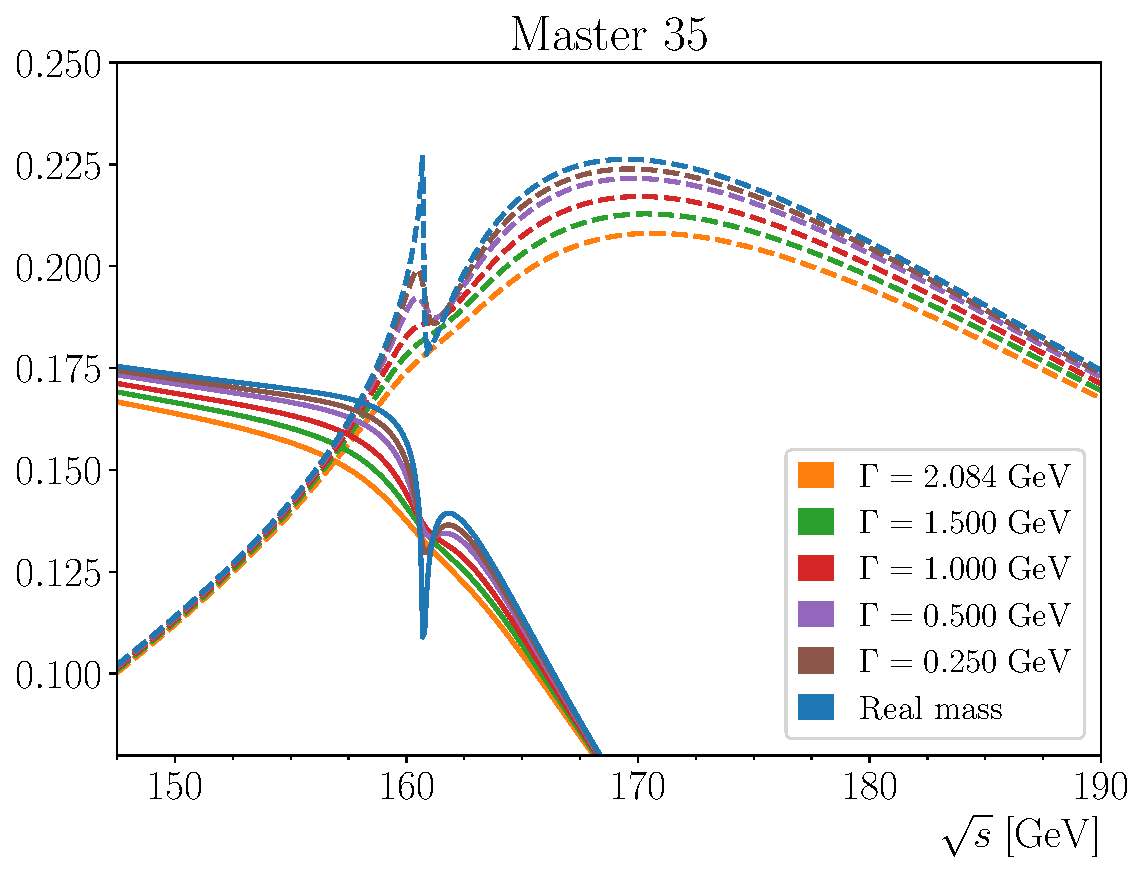
\includegraphics[width=0.7 \textwidth]{paperSeaFire/Images/master35_limit_final.pdf}
    \caption{Comparison between different values of the decay rate $\Gamma$ for MI35. The plot shows the value of the $\varepsilon^0$ order for $150\;\text{GeV}\le\sqrt{s}\le190\;\text{GeV}$ and $\cos{\theta}=0$ with the mass of the $W$ boson. The blue line corresponds to the real-valued mass case, while the other colours are for the complex-valued case with different $\Gamma$ values. The solid and dashed lines represent the real and imaginary part of the solution.}
    \label{fig:limit}
\end{figure}

The definition of the complex mass given in Eq.~\ref{eq:complex_mass} shows that the case of real masses can be thought also as the limit for $\Gamma\to0$. Hence, by considering values of $\Gamma$ gradually smaller, all the MIs should converge to the one obtained with real-valued internal masses. This is shown explicitly for MI35 in Fig.~\ref{fig:limit}, although it holds for all the other MIs. In particular we have compared the results for real- and complex-valued masses, where the latter have been calculated using different values of the decay-width $\Gamma$. In the plot we observe that all the lines approach the blue one, representing the real mass case, as expected.
We note that in the case of complex internal masses the dimensionless kinematic variables $(x,y)$ become complex. Hence, a Feynman prescription is not necessary, since we can always link two points in the complex plane in a consistent way, as described in Section~\ref{subsec:path}. On the contrary, when working with real-valued masses, $(x,y)$ may lay on a branch-cut, namely the real axis. In this case providing a Feynman prescription is mandatory for performing the analytic continuation in an unambiguous way. In conclusion, this example besides showing that \textsc{SeaSyde} can robustly handle arbitrary internal complex masses, indicates also that the complex mass scheme is consistent with the Feynman prescription, and, moreover, it can be used to automatically implement the causality of the theory.



\subsection{Checks and performances}

As anticipated in the previous section, we have checked our numerical results against other publicly available tools, namely \textsc{GiNaC}, \textsc{DiffExp}, \textsc{AMFlow} \cite{Liu:2022chg}. In particular, we have used \textsc{DiffExp} and/or \textsc{AMFlow} to check the value of the 36 MIs considering internal real-valued masses in all the regions of the phase space. We also have compared our results against \textsc{pySecDec} \cite{Borowka:2017idc}, but only in few points of the Euclidean region, with a limited number of significant digits.
We have used \textsc{GiNaC} to check the first 31 masters with internal complex-valued masses and arbitrary values of the Mandelstam invariants. The value of the last 5 MIs with internal complex masses is, instead, a new prediction. 

The strength of the series expansion approach is that we can achieve an arbitrary level of precision, by simply adding more terms in the expansion. The increase in precision, however, corresponds to an increase in the amount of time and computational resources necessary to carry out the calculation. The two aspects, hence, have to be carefully balanced.

As a check, we evaluated the MIs in different points of the phase space, below and above the thresholds at $\sqrt{s}=m_V$ and $\sqrt{s}=2 m_V$ and for different values of $\cos\theta$, using a different number of terms in the series. In particular, using $150$ terms, we have obtained perfect agreement between \textsc{SeaSyde}, \textsc{DiffExp} and \textsc{GiNaC} up to the 40th decimal digit, i.e. quadruple floating-point precision. 

Regarding the time performances, they strongly depend not only on the number of terms in the series, but also on the presence of singularities between the starting and ending points. In Table \ref{table:checks} we report the time necessary for transporting the boundary conditions from the Euclidean region to a test point, namely $\sqrt{s}=155$ GeV and $\cos\theta=0$, for different number of terms, along with the precision of the result.

\begin{table}[ht!]
    \centering
    \begin{tabular}{c c c}
    \toprule
    Number of terms & Precision & Execution time\\
    \toprule
    50 terms & $10^{-14}$ & $\sim 14$ min\\
    \midrule
    75 terms & $10^{-19}$ & $\sim 26$ min\\
    \midrule
    100 terms & $10^{-25}$ & $\sim 50$ min\\
    \midrule
    125 terms & $10^{-33}$ & $\sim 75$ min\\
    \midrule
    150 terms & $10^{-40}$ & $\sim 90$ min\\
    \toprule
    \end{tabular}
    \caption{Precision achieved and execution time for transporting the boundary conditions from the Euclidean region to $\sqrt{s}=155$ GeV and $\cos\theta=0$, for different number of terms in the series.}
    \label{table:checks}
\end{table}

This estimate is obtained on a MacBook Pro (2015) equipped with a 2.7 GHz Dual-Core Intel i5. The fact that the execution time increases so much with the number of terms, is mainly due to the poor-performances of the \textsc{Mathematica} function \texttt{Series} when dealing with series with a big number of terms. Anyhow, for most current precision studies, a $10^{-19}$ precision is sufficient. The execution time depends also on the distance between the starting point, where the boundary conditions are imposed, and the final one, in which we would like to evaluate the solution. For reaching the physical region we usually need a number between $15$ and $20$ steps. Given the results in Table \ref{table:checks} we can estimate a total of $50$, $160$ and $300$ seconds per step for $50$, $100$ and $150$ terms, respectively.
Once in the physical region, less singularities need to be avoided and, hence, more direct path can be chosen. In this case a number between $1$ and $10$ steps is sufficient to reach every point in the phase-space.

Given the time performances of our package, and in general of packages implementing the series expansion approach, a direct implementation in Monte Carlo generators is out of question.
However it is possible to reformulate the problem in such a way that an evaluation on-the-fly is not necessary: we can use {\sc SeaSyde} to obtain a numerical grid for the MIs first; a grid for the total correction can be computed later, covering the whole phase space of the process;
once this latter grid is ready, we can obtain the value of the correction at any point, simply by a linear interpolation, thanks to the smoothness of the total correction.
In Ref. \cite{Armadillo:2022bgm} we presented a numerical grid for the MI32-36. This grid is constituted by $(130\times25)$ points which samples the phase-space for different values of $(\sqrt{s},\cos\theta)$ in the range $\sqrt{s}\in [40,13000 ] $ GeV and $\cos\theta\in[-1,1]$. The full evaluation was performed in parallel on 26 cores on an Intel Xeon Silver 4110 2.1 GHz, considering $75$ terms, and took 11 hours in total. 